\documentclass[review]{elsarticle}

\usepackage{hyperref}
%\usepackage{lineno,hyperref}
%\modulolinenumbers[5]

\journal{Optics Communications}

%%%%%%%%%%%%%%%%%%%%%%%
%% Elsevier bibliography styles
%%%%%%%%%%%%%%%%%%%%%%%
%% To change the style, put a % in front of the second line of the current style and
%% remove the % from the second line of the style you would like to use.
%%%%%%%%%%%%%%%%%%%%%%%

%% Numbered
%\bibliographystyle{model1-num-names}

%% Numbered without titles
%\bibliographystyle{model1a-num-names}

%% Harvard
%\bibliographystyle{model2-names.bst}\biboptions{authoryear}

%% Vancouver numbered
%\usepackage{numcompress}\bibliographystyle{model3-num-names}

%% Vancouver name/year
%\usepackage{numcompress}\bibliographystyle{model4-names}\biboptions{authoryear}

%% APA style
%\bibliographystyle{model5-names}\biboptions{authoryear}

%% AMA style
%\usepackage{numcompress}\bibliographystyle{model6-num-names}

%% `Elsevier LaTeX' style
\bibliographystyle{elsarticle-num}
%%%%%%%%%%%%%%%%%%%%%%%

\usepackage{float}
\usepackage{amssymb}
\usepackage{graphicx}
\usepackage{amsmath}%
\usepackage{amsfonts}%
\usepackage{graphicx}
\usepackage{cancel}
\usepackage{hyperref}
\usepackage{algorithm}
\usepackage{algpseudocode}
\usepackage{multirow}
%\usepackage{subfig}
\usepackage{tabularx}
\usepackage{subfigure}
\usepackage{mathtools}
\usepackage{setspace}  
\usepackage{epsfig}

\begin{document}

\begin{frontmatter}

\title{Parallel Demodulation Algorithm for Processing Independent Windows of a Fringe Patterns Using Simulating Annealing}

%% Group authors per affiliation:
\author[cio]{I. Mor\'e \corref{cor1}} 
\ead{imore@cio.mx}
\author[cio]{F. J. Cuevas}
\ead{fjcuevas@cio.mx}
\author[cidesi]{J. Jimenez}
\ead{fer\_vielma@yahoo.com}

\address[cio]{Centro de Investigaciones en \'Optica, A.C.\\ Loma del Bosque 115, Colonia Lomas del Campestre 	Le\'on, Guanajuato CP 37150}
\address[cidesi]{Centro de Ingenier\'ia y Desarrollo Industrial, \\ 	Alianza Sur No. 203. Autopista al Aeropuerto Km. 10
	Apodaca N. L.}

\cortext[cor1]{Corresponding author}
% \tnotetext[mytitlenote]{Fully documented templates are available in the elsarticle package on \href{http://www.ctan.org/tex-archive/macros/latex/contrib/elsarticle}{CTAN}.}

% %% Group authors per affiliation:
% \author{Elsevier\fnref{myfootnote}}
% \address{Radarweg 29, Amsterdam}
% \fntext[myfootnote]{Since 1880.}

% %% or include affiliations in footnotes:
% \author[mymainaddress,mysecondaryaddress]{Elsevier Inc}
% \ead[url]{www.elsevier.com}

% \author[mysecondaryaddress]{Global Customer Service\corref{mycorrespondingauthor}}
% \cortext[mycorrespondingauthor]{Corresponding author}
% \ead{support@elsevier.com}

% \address[mymainaddress]{1600 John F Kennedy Boulevard, Philadelphia}
% \address[mysecondaryaddress]{360 Park Avenue South, New York}

\begin{abstract}
It is presented a method for demodulating fringe patterns, which uses the Simulated Annealing algorithm by setting an objective function, and it is capable of recovering the phase map without using a unwrapping algorithm. This method is based on the window fringe pattern demodulation method and introduces an recursive algorithm that performs an automatic partitioning of the pattern of fringes using quad tree data structure and limiting a maximum number of fringes in each partition. The phase is approximated by means of a parametric estimation of a polynomial of the \textit{n}-th degree in each window independently, which facilitates parallel implementation and ultimately a gain in speed. The computer simulation and the experimental results have demonstrated that this method is able to recover the phase map in complex interferograms with results comparable to the soft computing techniques that address this problem ( Independent
Windows Using a Genetic Algorithm), with regards to quality of results, furthermore it presents a parallel implementation which makes the demodulation process more agile.
\end{abstract}

\begin{keyword}
Interferogram \sep Simulating Annealing \sep Demodulation \sep Fringe Patterns
\MSC[2019] 00-01\sep  99-00
\end{keyword}

\end{frontmatter}

%\linenumbers

\section{Introduction}

In Optical Metrology, the phase extraction from a single interferogram is important for interferometric applications, where it is necessary to measure of a wide range of physical quantities, however, it is consider a difficult problem, especially in transcient experiments and when there is a subsampling of the fringes.

Generally, a fringe pattern can be considered as a fluctuation of a sinusoidal signal in the bi-dimensional space, which is related to the physical quantity being measured. The mathematical model that characterizes a fringe pattern $I(x,y)$ can be formulated as:
\begin{equation} \label{eq1}
    I(x,y) = a(x,y) +b(x,y)cos(\phi(x,y)) + n(x,y),
\end{equation}
where the term $a(x,y)$ represents background lighting, $b(x, y)$ refers to contrast or modulation of the signal, related to the reflectance of the object, $\phi(x,y)$ is the phase term, which is related to the physical amount that is quantified, and $n(x, y)$ represents high-frequency noise.

Among the methods used to calculate the phase term, the most popular are the Phase-Shifting (PS) \cite{malacara2007optical,Kujawinska1991} and Fourier method (FM) \cite{Takeda:82,Takeda:83}. Phase-shifting is a powerful technique in optical metrology to measure a wide variety of physical quantities, unfortunately, this algorithm requires at least three interferograms with known phase shifts.  This requirement may be unpractical in some experiments, such as transient mechanical processes or in testing with acquisition of multiple interferograms without disturbance.

On the other hand, Fourier transform is a global method, that can recover the phase from a single interferogram, but has the disadvantage that only analyze patterns of open fringes \cite{Takeda:82} and usually the global phase is too complex to be mathematically represented \cite{Bone:86}. Moreover, this method estimate the phase wrapped because of the arctangent function used in the phase computation, consequently  needs a phase development algorithm, and also requires the design of a filter to obtain the phase.

In recent years, many phase recovering methods have been developed to reconstruct the phase maps from single open or closed fringe patterns \cite{Servin:03,Robin:04,Robin:05,Rivera:05,Estrada:07,Kemao:07,Dalmau-Cedeno:08,Dong:16,Trusiak:16,Feng2019,Jin-Min2019,Munoz2019}, such as regularized phase tracing (RPT) \cite{Tian:10,Servin:97}, which is one of the most robust and effective methods but, it often fails in the cases  of complex interferograms and needs well-defined scanning strategies. In a recent work, Kai \cite{Kai:12} presented two novel improvements for RPT technique, which can directly demodulate a single fringe pattern without any pre-processing and post-processing and successfully get rid of the problem of the sensitivity to critical points. A disadvantage of this is lengthy calculation time, specially designed scanning strategy, and sign-ambiguity problems caused by noise and saddle points reduce its effectiveness, especially for demodulating large and complex fringe patterns \cite{He:17}.

Novel methods use soft computing algorithms like neural networks and optimization algorithms. Among the main approach that use the neural network technique is the works presented by Cuevas \cite{CUEVAS2000239,CUEVAS1999270}, where a multilayer neural network is trained by using fringe patterns and the phase gradients associated with them, from calibrated objects. Methods using optimization model  approximate the phase through the estimation of parametric functions, for example soft computing techniques applied to Zernike polynomials \cite{Espinosa2007a,Tian:11}, combination of Genetic Algorithms and parametric methods \cite{Cuevas2002,Cuevas2006a,Toledo2008}, Particle Swarm Optimization \cite{Jimenez2012} and, Harmony Search Optimization \cite{articleFDO}, among others.

In the present paper, a method is proposed to obtain a parametric approach, using the Simulated Annealing (SA) technique, to determine the phase term ($\phi(x,y)$) from a single fringe pattern using parallel computing. This method represents a modification of the Fringe Processing on Independent Windows (FPIW) \cite{Toledo2008} to demodulate complicated fringe patterns using SA  to fit a polynomial on sub-sampled images. The SA technique was introduced with the aim of improving the processing time by parallel process implementing a model for partitioning in order to ensure the same level of complexity in each window partition using a quad tree data structure.

The paper is organized as follows. In Section 2. will be presented methodology and design of a Parallel Demodulation Algorithm for processing of a Fringe Patterns. Results and discussions will be given in Section 3. In section 4. the conclusions will be reached.

\section{Parallel Demodulation Algorithm for processing of a Fringe Patterns}

In the proposed method, fringe pattern normalization process is necessary, that is why normally, the information contained in fringe patterns is confined in the modulating phase, mainly images obtained in real experiments, which are subjected to image processing to eliminate the noise, and then images are binarized, thus guaranteeing the efficiency of the splicing procedure.

After background suppression and modulation normalization, the resolution of the fringe pattern is reduced, to increase the speed of the search process; and following, is partitioned using a quad tree data structure where each leaf represents a independent sub-images that contain a number of fringes less than or equal to a value provided as a parameter. Then, a polynomial function is fitted to approximate the phase field of each window using SA. This procedure is applied in parallel over all sub-images in the window partition. At the end, a splicing procedure is required to connect different SA fitted phase windows and determine the whole phase field $\phi(x,y)$. The complete demodulation process is overriding in the next subsection.

\subsection{Algorithm for Automatic Partition of an Interferogram (API) in independent windows.}

One of the main contribution of this work is based on implementing on window partition algorithm \cite{Cuevas2006a}, that is used to divide an interferogram with a maximum limit of fringes in each window. This process consists of obtaining the lowest amount of sub-images consistent with the number of allowed fringes. For this purpose, a tree-type data structure was implemented \cite{goodrich2004data}, where each leaf of the tree represents a partition of the interferogram. Fig.\ref{Fig1} shows the general scheme of the employed data structure.
\begin{figure}[ht]
    \centering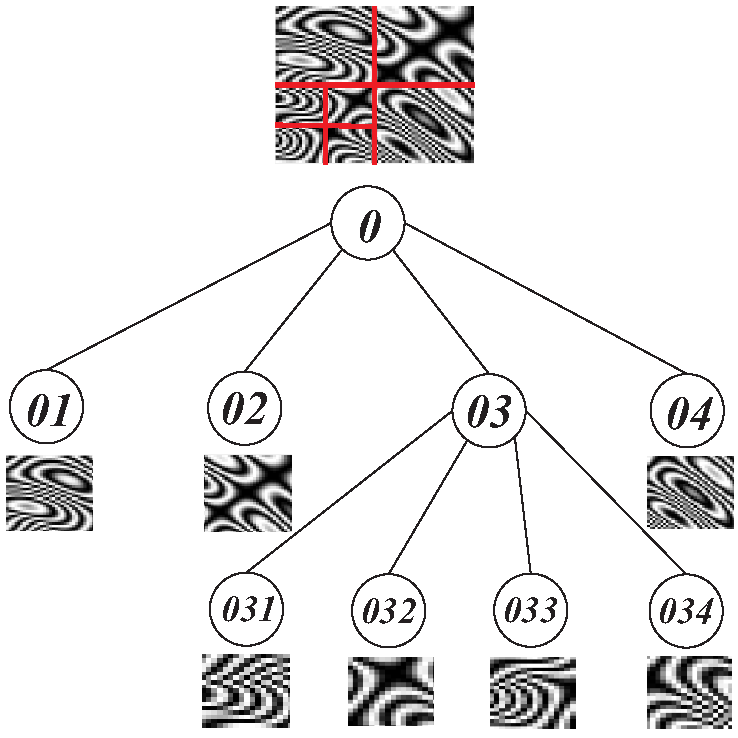
\includegraphics[width=10cm]{fig1}
	\caption{Diagram of the data structure used to store the windows of the interferograms divided by the algorithm.}
 	\label{Fig1}
\end{figure}

API is a recursive method that implements a post-order traversal and verifies that each sheet complies with the number of fringes restriction. The algorithm verifies if the node has a child, and if so, the recursive method with all the children is called again. Otherwise, the node is a leaf, and it is verified whether it complies with the number of fringes restriction. If it does the process for that window is stopped; otherwise, the interferogram is partitioned into 4 sub-images. The process is repeated until all sheets have the maximum number of required fringes. Algorithm \ref{IPA} shows the pseudo-code for API.
 
 \begin{algorithm}[H]
	\caption{API Algorithm}\label{IPA}
	\begin{algorithmic}[1]
		\Procedure{WinPartitionR}{}
		\State \textbf{Input:}
		\State $Nodo \to \textit{Interferogram Partition}$
		\State $N \to \textit{Fringes Number}$
		\State $Tree \to \textit{Data Structure}$
		\If {Nodo != null}
		\State $FirstSon = Nodo.getFirst\_Son$
		\While{FirstSon != null }
		\State $FirstSon = FirstSon.getFollow\_Brother$
		\State $WinPartitionR(FirstSon, N, Tree)$
		\EndWhile
		
		\If {Nodo.getFirst\_Son == null}
		\If {Nodo.getFringes \textgreater \ N}
		\State $arraySons = Partition(Nodo)$
		\State $Tree.add(arraySons)$
		\EndIf
		\EndIf
		\EndIf
		
		\State $\textbf{Output:}\ Tree$	
		\EndProcedure
	\end{algorithmic}
\end{algorithm}
\subsection{Simulated Annealing}

The SA technique was formulated by Kirkpatrick, et al in 1983 \cite{metropolis1953,Kirkpatrick1983}, based on the Monte Carlo method for estimating the properties of any material or substance made up of individually interacting molecules.

The SA begins with a randomly generated  initial solution. Generally, the algorithm starts with a high temperature, which is reduced according with the cooling schedule. At each temperature level, several neighboring solutions ($nrep$) are explored, which are accepted if they exceed objective function of the initial solution, otherwise  a new solution is accepted with a certain probability. The process is repeated until a stop condition is fulfilled.

\subsection{Parallel analysis of fringe patterns using a Simulated Annealing  algorithm}

The analysis of fringe patterns mainly focuses on the precision, automaticity, and speed. There are 2 ways to accelerate the speed of an algorithm, the first one is decreasing the computational complexity of the algorithm by means of parallelism or using the philosophy of divide and conquer, and the second by hardware.

The presented technique aims to address the concept of parallel computing and its applications in the analysis of fringe patterns by modeling the problem in such a way that it can be divided into \textit{n} independent tasks. As mentioned in the previous section a fringe pattern is partitioned into independent windows, which are fitted to approximate the phase field of each sub-image by means of a parametric function. A SA is used to find the function's parameters by the optimization of an Objective Function ($F$) \cite{Cuevas2002}. The fitness function is composed of two terms: the first term refers to the fringe similarity criterion and the second indicates the smoothness criterion where the sum of the cross-gradients that yield soft solutions is penalized. When the information about the shape of the object $\phi(x, y)$ is unknown, a polynomial adjustment is recommended. An $F$ for each sub-image is used to obtain the fitness value, it can be written as:
\begin{eqnarray} \label{eq2}
F &=& \sum_{y=1}^{R} \sum_{x=1}^{C} \bigg\lbrace\ \big(\ I(x,y) - (128 -127\cos\left[\phi(x,y)\right])\ \big)^2 \nonumber  \\ 
&+& \mu\big [\big(\phi(x,y) - \phi(x+1,y+1) \big)^2  + \big(\phi(x+1,y) - \phi(x,y+1) \big)^2\big ] \bigg\rbrace \text{,}
\end{eqnarray}
where $x$ and $y$ are integer values that indicate the position of the pixels in the interferogram, $\mu$  is the softness parameter which implies a smoother adjustment function is obtained for a higher value of the $\mu$ parameter, $I(x, y)$ is the intensity value detected at the point $(x, y)$ and $\phi(x, y)$ represents the two-dimensional polynomial approximation of degree $n$ which during the optimization process given by:
\begin{eqnarray}\label{eq3}
\phi(x,y) = s_0+s_1 x+s_2 y+s_3 xy+s_4 x^2+s_5 y^2 +\dots + s_{\frac{(n+1)(n+2)}{2} - 1} y^n\text{,}
\end{eqnarray}
where the terms $s_i$ represent the coefficients of the polynomial that approximate the phase term.

\subsubsection{Initial solution}

For this study, random generation of the initial solution $S$ is used, which is  a vector of \textit{n-}parameters, where each $s_i$ term indicates a coefficient of a possible approximation, from Equation \ref{eq3}:
\begin{equation}
S = \left[ s_0, s_1, s_2,\ldots,s_{\frac{(n+1)(n+2)}{2}}\right] \text{,}
\end{equation}
where each $s_i$ term is a real value within a range defined by the user $[Inf_i, Sup_i]$. These values can be taken from prior knowledge, if it is available.

To define the search interval it is necessary to involve the a priori knowledge of the problem in question. It is known that the equation that models an interference pattern has a cosine profile which indicates that between each maximum or minimum of the cosine function there are $2\pi$ radians, this means, in each interval of $2\pi$ radians there are one white and one black fringe. This implies that each term $a_i$ contributes to the total of radians within the fringe pattern which is related by:
\begin{equation}\label{eq4}
\max(\phi(x,y)) - \min(\phi(x,y)) = 2\pi N \text{,}
\end{equation}
where $F$ represents the number of interferogram fringes.

Assuming the maximum values of the variables $x$ and $y$, it can find the interval of each coefficient from the following mathematical statements:
{
	\begin{eqnarray}\label{eq4.2}
	&s_0& = 2\pi F \ \to s_0\in\left[-2\pi F, 2\pi F\right] \text{,}\nonumber \\[0.3cm] \nonumber
	&s_1& = \frac{2\pi F}{X_{max}} \ \to s_1\in\left[-\frac{2\pi F}{X_{max}}, \frac{2\pi F}{X_{max}}\right] \text{,}\\[0.3cm]\nonumber
	&s_2& = \frac{2\pi F}{Y_{max}} \ \to s_2\in\left[-\frac{2\pi F}{Y_{max}}, \frac{2\pi F}{Y_{max}}\right]  \text{,}\\[0.3cm]\nonumber
	&\hspace{6cm} \vdotswithin{\mspace{-300mu}} \qquad \vdotswithin{\mspace{-300mu}} \nonumber\\[0.3cm]
	&s_{\frac{(n+1)(n+2)}{2}-1}& = \frac{2\pi F}{(Y_{max})^n} \ \to s_n\in\left[-\frac{2\pi F}{(Y_{max})^n}, \frac{2\pi F}{(Y_{max})^n}\right]\text{,}
	\end{eqnarray}
}
where $Y_{max}$ and $X_{max}$ represent the number of rows and columns of the fringe pattern.

\subsubsection{Neighborhood solution}

One of the factors that influence the efficiency of the SA algorithm is the vicinity function used during the optimization process \cite{Moscato:1993}. The objective of the vicinity function is to provide a solution $S_{i+1}$ through an operator of movements, which slightly alters the solution $S_i$. For this purpose, it is necessary to establish how to get the solutions that make up the vicinity given a particular solution and how to select one of them as a candidate for a new solution.  In this work, a greedy search is performed to generate $\frac{(n+1)(n+2)}{2}-1$ neighboring solutions. New local solutions are generated by varying each coefficient $s_i$ of the initial solution and thus obtaining a neighborhood from which the best element is selected. The current coefficients $s_i$  are modified using the following equation:
\begin{equation}\label{eq5}
s_i = s_i + rand( \alpha_i*Inf_i,\ \alpha_i *Sup_i) \text{,}
\end{equation}
where $rand(a, b)$ generates a random number with a uniform distribution in the range $[a, b]$, $Sup_i$ and $Inf_i$ represent the upper and lower limits of the allowable space for each coefficient, respectively, and $\alpha$ is a variable parameter that depends on the Boltzmann temperature function ($\alpha_i = \frac{T_i}{T_0}$), because its objective is to delimit the interval of each coefficient and just as the temperature function, $\alpha_i$ decrements the interval in each iteration. In addition, if a coefficient exceeds the definition limits, it is penalized and a new random value is generated in the allowable space.

\subsubsection{Cooling schedule and stop conditions}

The cooling scheme in the SA must provide a compromise between the execution time and the quality of the final solution. There are several studies focused on cooling programs, among which are noteworthy \cite{cardoso1994nonequilibrium} and \cite{nourani1998comparison}. In this case, a function is defined which ensures that the temperature gradually decreases with the number of iterations ensuring that the temperature reaches its minimum value in the last iteration. The following equation shows the implemented temperature function:
\begin{equation}\label{eq6}
T(i) = e^{-10^{-6}*i^2 + \frac{log(\frac{10*T_{f}}{T_{0}})}{N} + N*10^{-6} + log(T_{0}) } \text{,}
\end{equation}
where $i$ represents the current iteration, $N$ the number of iterations, $T_{0}$ and $T_{f}$ indicate the initial and final temperatures of the model. For instance, having  $N = 500$, $T_{0} = 9\ 000$ y $T_{f} = 1$, Equation \ref{eq6} has the following behavior, shown in Fig. \ref{Fig2}. The temperature function is related to the number of iterations and the limits of desired temperature, the SA does not stop until both conditions are met.
\begin{figure}[ht]
\centering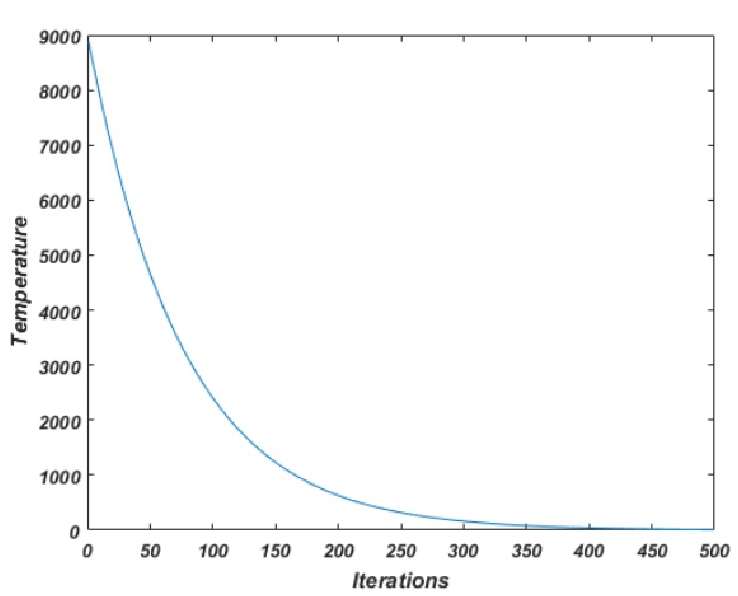
\includegraphics[width=8cm]{fig2}
\caption{Graph of temperature function $T(i)$ from Eq. \ref{eq6}.}
\label{Fig2}
\end{figure}

\subsection{Unification of the phase from the independent windows.}

The phase demodulation is achieved by window segmentation of the fringe pattern and is executed in separate tasks and in parallel. The splicing procedure used constitutes an improvement of the method presented in \cite{Toledo2008} because it avoids the use of overlapping regions in neighboring windows. The phase window unification algorithm is composed of the following steps:
\begin{enumerate}
	\item The phase of the first window adjusted by SA is taken as reference.
	\item The neighboring phase $(\phi(x,y)$ is selected and its phase is calculated with inverted concavity $(\phi(x,y)')$. 
	\item The modification consists in that the overlapping region that will be chosen from the reference image will be done by polynomial approximation using cubic spline \cite{burden2002analisis}. In other words, if the bordering region of the reference phase is the last row or column, or both; extrapolation is done to find the $n + 1$ row or column corresponding to the current phase. Fig. \ref{Fig3} shows a proceeding and scheme of the extrapolation process.
		\begin{figure}[ht]
		\centering
		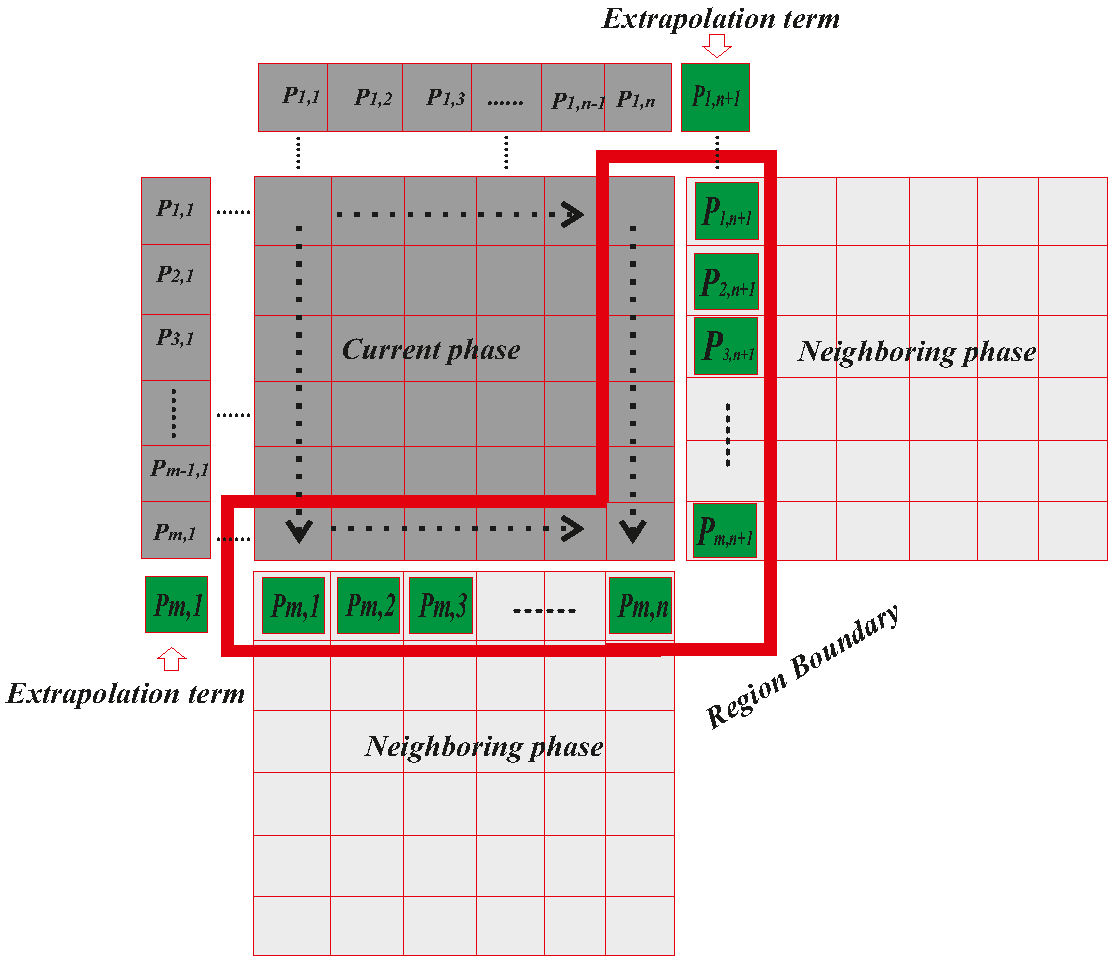
\includegraphics[width=8cm]{fig3}
		\caption{Border region between neighboring phase maps.}
		\label{Fig3}
	\end{figure}
The $DC$ or height difference between the frontier region for $\phi(x,y)$ and $\phi(x,y)'$ is calculated by the following expressions:
	\begin{eqnarray}\label{eq7}
	DC_1= \frac{\sum_{x,y\in N}(\varTheta(x,y) -\phi(x,y))}{A} \text{,}\nonumber \\
	DC_2= \frac{\sum_{x,y\in N}(\varTheta(x,y) -\phi(x,y)')}{A} \text{,} 
	\end{eqnarray}
	where $\varTheta(x,y)$ is the region extrapolated by spline cubic, $N$ is the region border and $A$ is the area $(pixel^2)$ of the region.	
	\item The mean squared error for both alternatives is calculated as follows with the aim of making a comparison between both. 
	\begin{eqnarray}\label{eq8}
	RMS_1= \frac{\sum_{x,y\in N}(\varTheta(x,y) -\phi(x,y) - DC_1)^2}{A} \text{,} \nonumber \\
	RMS_2= \frac{\sum_{x,y\in N}(\varTheta(x,y) -\phi(x,y)'-DC_2)^2}{A} \text{,} 
	\end{eqnarray}
The phase with the lowest RMS will be displaced by a value of $\phi(x,y) + DC1$ or $\phi(x,y)' + DC2$ to place it at the level of the reference phase map.
	\item The process is repeated until each phase map has been moved.
\end{enumerate}

\section{Experimental results and Computer Simulation}

The proposal method was tested with several experiments including computer simulated patterns and real images obtained from an experimental arrangement.The first experiments correspond to the computer simulated fringe pattern proposed in \cite{Toledo2008}. The fringe pattern was sampled to produce an image of 54 $\times$ 54 pixels (Fig. \ref{Fig4}-a) and  the result of applying the  API algorithm using a maximum number of fringes per window equal to 3 is shown in Fig. \ref{Fig4}-b.
\begin{figure}[ht!]
\centering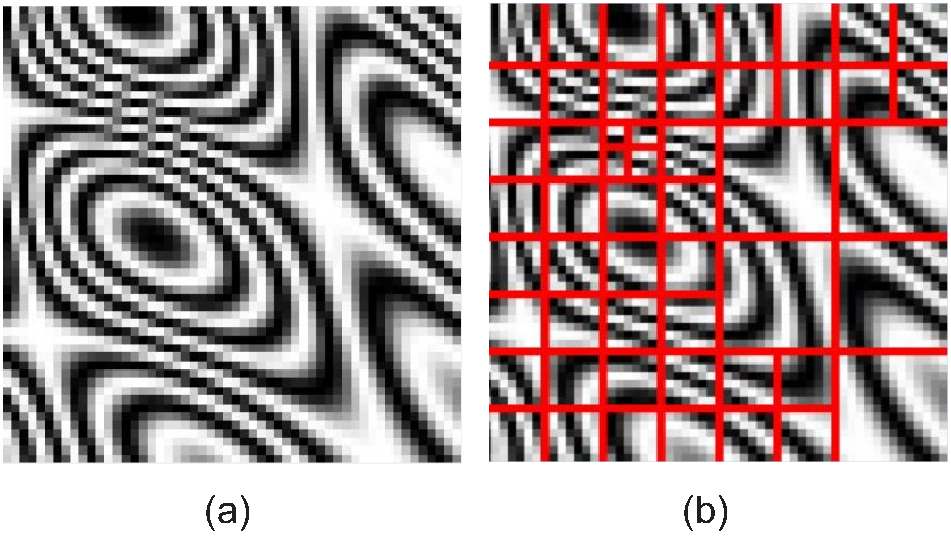
\includegraphics[width=8cm]{fig4}
\caption{(a) Sampled fringe pattern 54 $\times$ 54 pixel. (b) Result of the automatic partition obtained by API.}
\label{Fig4}
\end{figure}

A third degree polynomial was used to interpolate every partition. The values of the parameters used to achieve SA convergence were: generation numbers($N$) of 300, starting temperature $T_0 = 11 000$, the softness factor $\mu = 5$ and the number of neighboring solutions generated at each temperature level was 175. All the experiments were tested in a standard node that has 24 cores (2 sockets Intel Xeon E5-2680 v3 at 2.5 Ghz with 12 cores per socket) and 128 GB of shared RAM.

The resulting fringe pattern and the map phase recovered by the method are shown in Fig. \ref{Fig5}-a and \ref{Fig5}-b. For illustrative purposes, the difference between the computer simulated phase map and the one obtained during demodulation is shown in Fig. \ref{Fig5}-c. The root mean square (RMS) was used to measure the differences between simulated phase map and the one predicted by the model. RMS error is 0.007 rad, this measurement is 22 times lower than the reported in \cite{Toledo2008} of 0.154 rad.
\begin{figure}[ht!]
\centering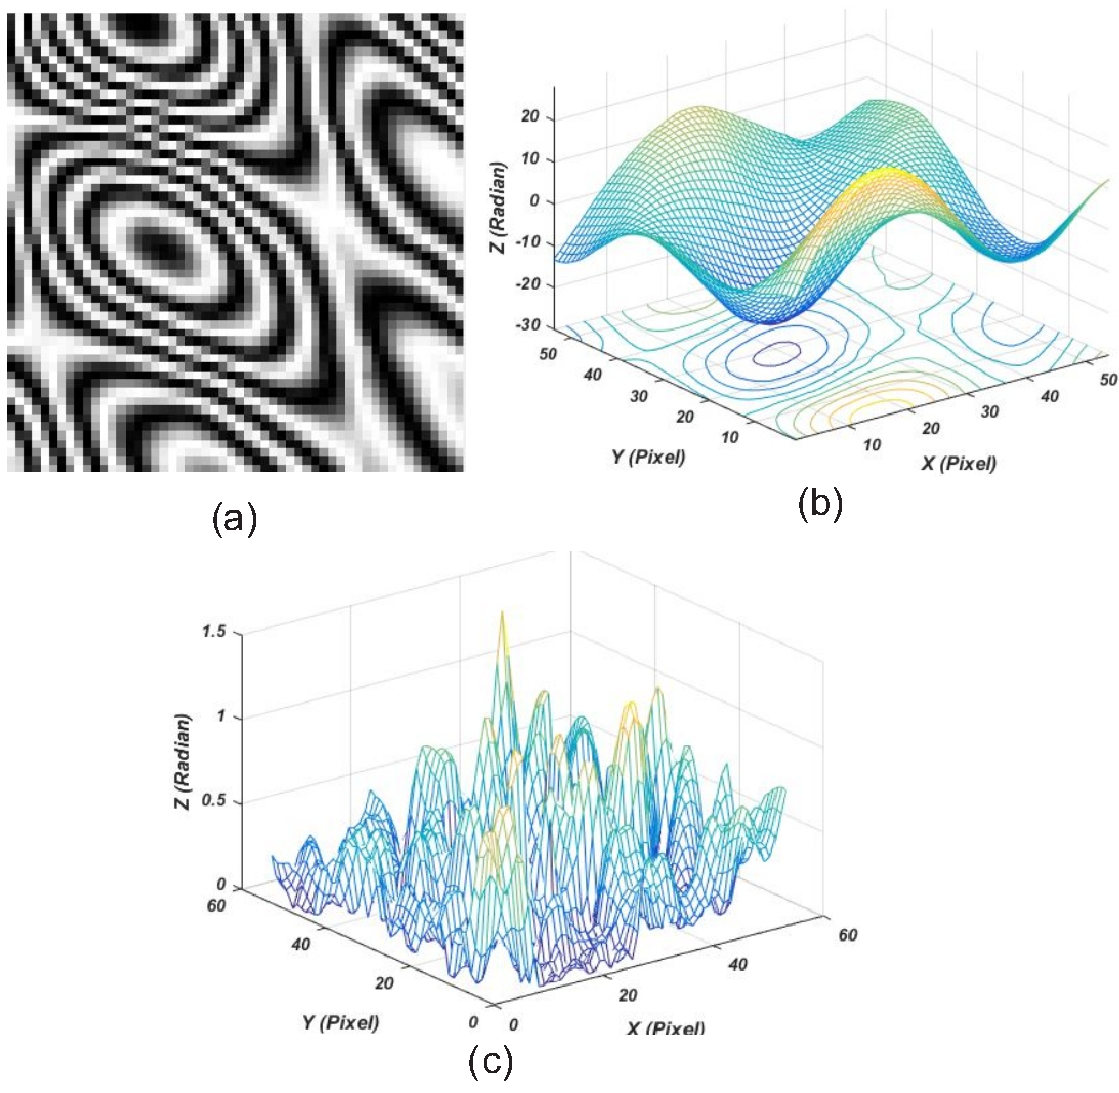
\includegraphics[width=10cm]{fig5}
\caption{(a) Fringe pattern recovered by the method. (b) Phase map demodulated. (c) Error graph between original and demodulated phase.}
\label{Fig5}
\end{figure}

Doing a comparative analysis with the model proposed by Toledo in \cite{Toledo2008}, the proposed method is able to obtain the phase map with a lower RMS value, in addition to introducing a new model of window partition based on the frequency of the fringes per partition facilitates the use of the same configuration of SA parameters for each window. Another aspect to compare is that the proposed method does not use the concept of overlapped region between neighboring windows bringing as an advantage that the same region is demodulated more than once.The last criterion taken into comparison was the speed factor. Assuming that both algorithms are executed in similar conditions, the number of evaluations of the objective function of the method proposed by \cite{Toledo2008} exceeds in approximately $2.85$ times the number of evaluations of the model proposed for a single window, all this without taking into account the time of selection, crossing and mutation of the genetic algorithm. In addition, the proposed model has a parallel implementation as opposed to the serial implementation of \cite{Toledo2008}, which increases its superiority in demodulation time used in \cite{Toledo2008}.

The second experiment consisted of approximating a computer simulated interferogram where the mathematical model of the original phase map is given by:
\begin{eqnarray}\label{eq9}
	f(x,y) = (0.1x - 0.02y + 0.01xy -0.02x^2)cos(\frac{x+y}{8});\\
	  x\in[-32, -10] \ \text{and} \ y\in[-15, 20].\nonumber
\end{eqnarray}

The objective of this experiment is to demonstrate the ability of the algorithm to recover phase in low resolution interferograms, even when the Nysquist criterion is not met. The computer simulation was reduced to a resolution of 36 $\times$ 36 pixels to be used as input to the algorithm and to apply an automatic partitioning with a maximum number of fringes equal to 5.  The result of applying the API algorithm is shown in Figure \ref{Fig6}(a).
\begin{figure}[ht!]
\centering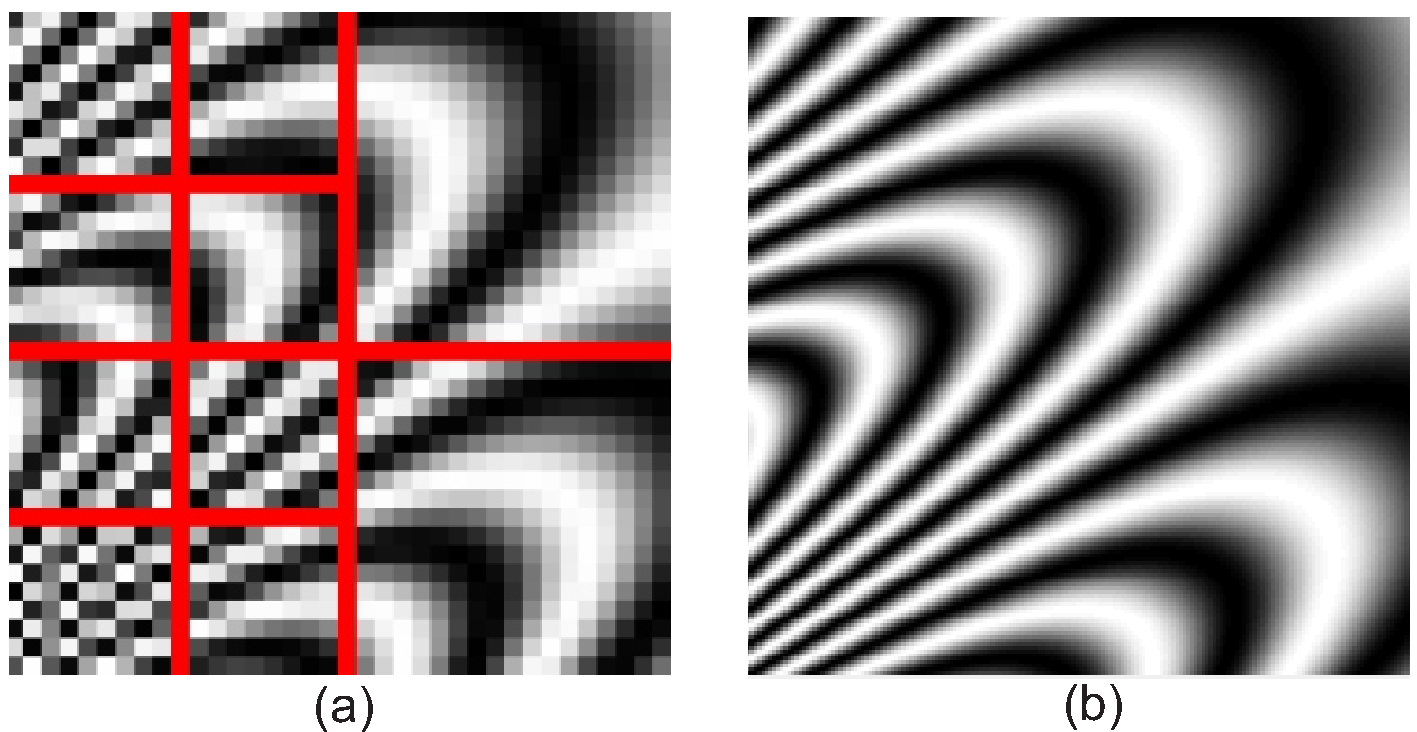
\includegraphics[width=10cm]{fig6}
\caption{(a) Result of the automatic partition obtained by API in low resolution. (b) Fringe pattern simulated in high resolution (156 $\times$ 156 pixels).}
\label{Fig6}
\end{figure}

Phase demodulation is achieved by segmenting the  fringe pattern windows using SA for each window independently, so this process is carried out in parallel. Each window was demodulated by adjusting a third degree 3 polynomial during 200 iterations with a generation of 50 neighboring solutions at each temperature level for a time of 109 seconds. The values of the initial temperature and the softness factor were 9000 and 15 respectively.

The resulting fringe pattern related to the demodulated phase and a comparison between both phase maps in high resolution are shown in Figure \ref{Fig7}. The root mean square (RMS) between the two phase maps was of 0.0073.
\begin{figure}[ht!]
\centering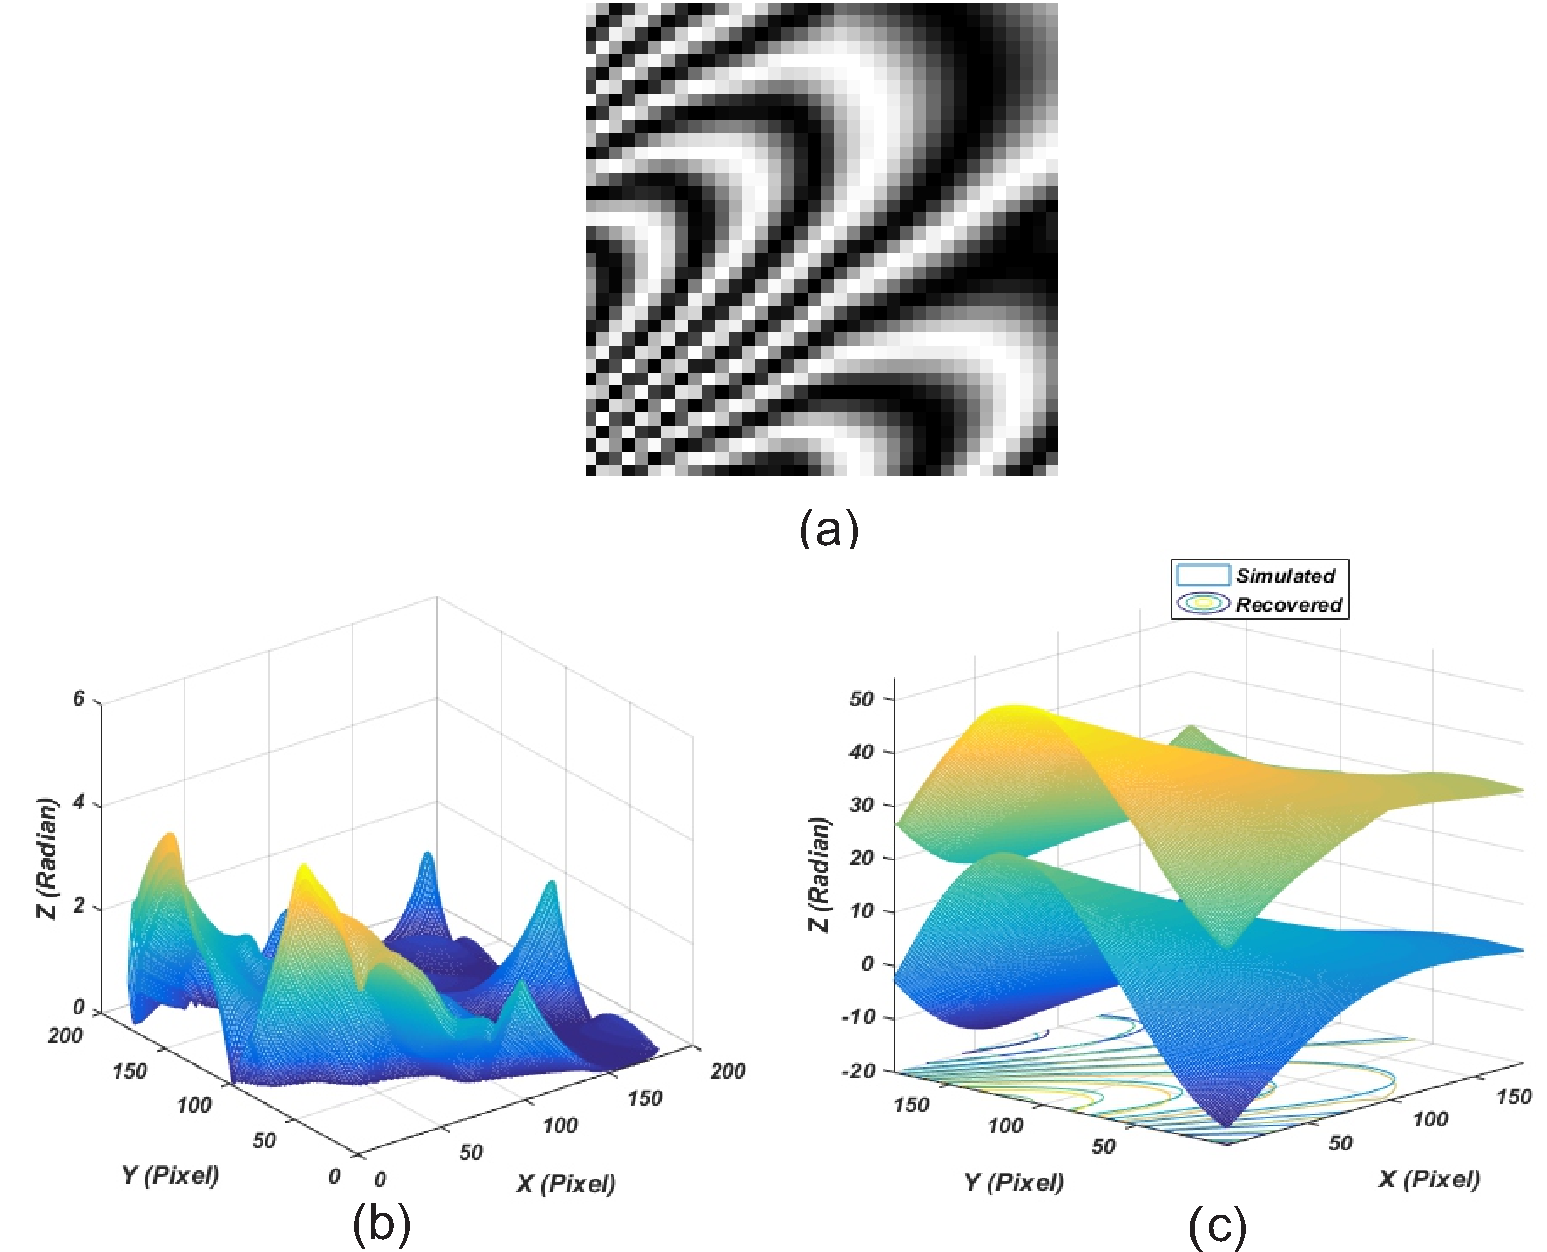
\includegraphics[width=10cm]{fig7}
\caption{(a) Fringe pattern recovered by the method. (b) Error graph between original and demodulated phase in high resolution. (c)Phase map demodulated and simulated in high resolution.}
\label{Fig7}
\end{figure}

The third interferogram taken into account in the experimental validation corresponds to a fringe pattern obtained from a shadow Moire experiment (Figure \ref{Fig8}a). A hemi-spherical object was located behind a Ronchi ruling and was illuminated by a collimated haze. To reduce the search space of the algorithm, the resolution of the interferogram was reduced to 37x43 pixels and the image was binarized using the Otsu method \cite{1979:ots} in small neighborhoods to ensure that background illumination and amplitude modulation were constant; and later was partitioned by the API algorithm using a maximum number of fringes per window equal 4 (Figure \ref{Fig8}b). The binarization process was performed in each window independently due to the different contrast variations in different positions product of the lighting.

\begin{figure}[ht!]
\centering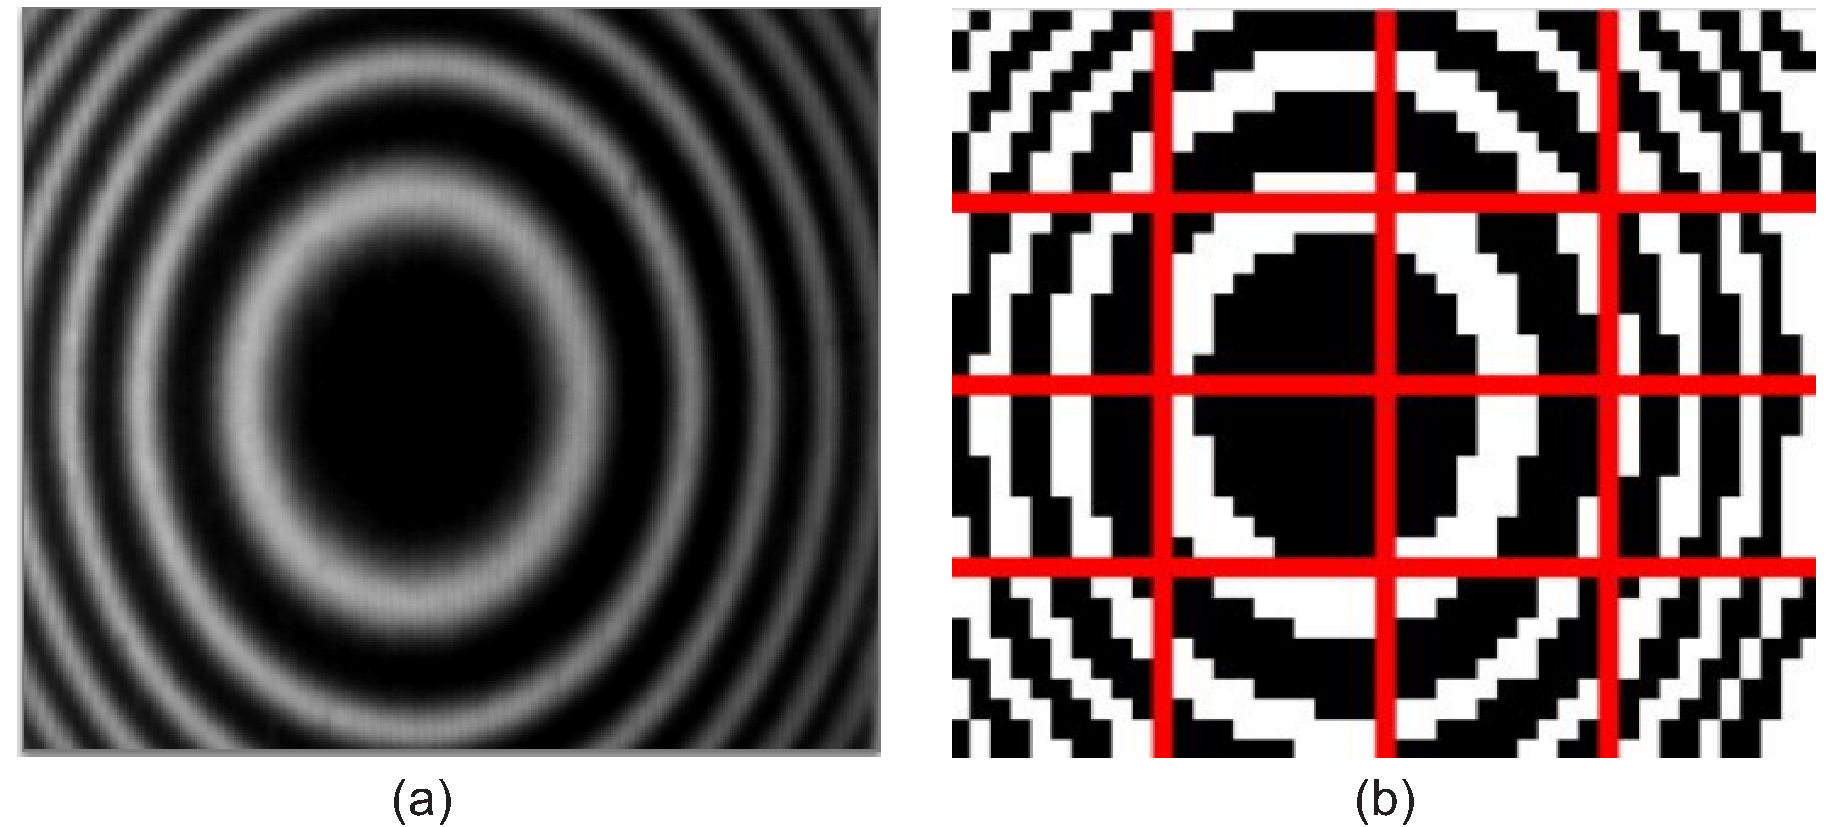
\includegraphics[width=10cm]{fig8}
\caption{(a) The shadow fringe pattern generated by a hemi-spherical object with resolution of 244 $\times$ 281 pixels. (b) Independent windows partition carried out by IPA.}
\label{Fig8}
\end{figure}

 The SA algorithm evolved during 3000 iterations to fit a second-degree polynomial to each sub-image in a period of 29 seconds. Thirty neighbors were generated in each iteration, the initial temperature used was 900, and the softness factor was 5.  Figure \ref{Fig9} show the results obtained by the demodulation process. It is worth noting that the phase map obtained after applying the unification algorithm of the windows, a low-pass filter was applied to eliminate the roughness between the limits of the windows.
  \begin{figure}[ht!]
\centering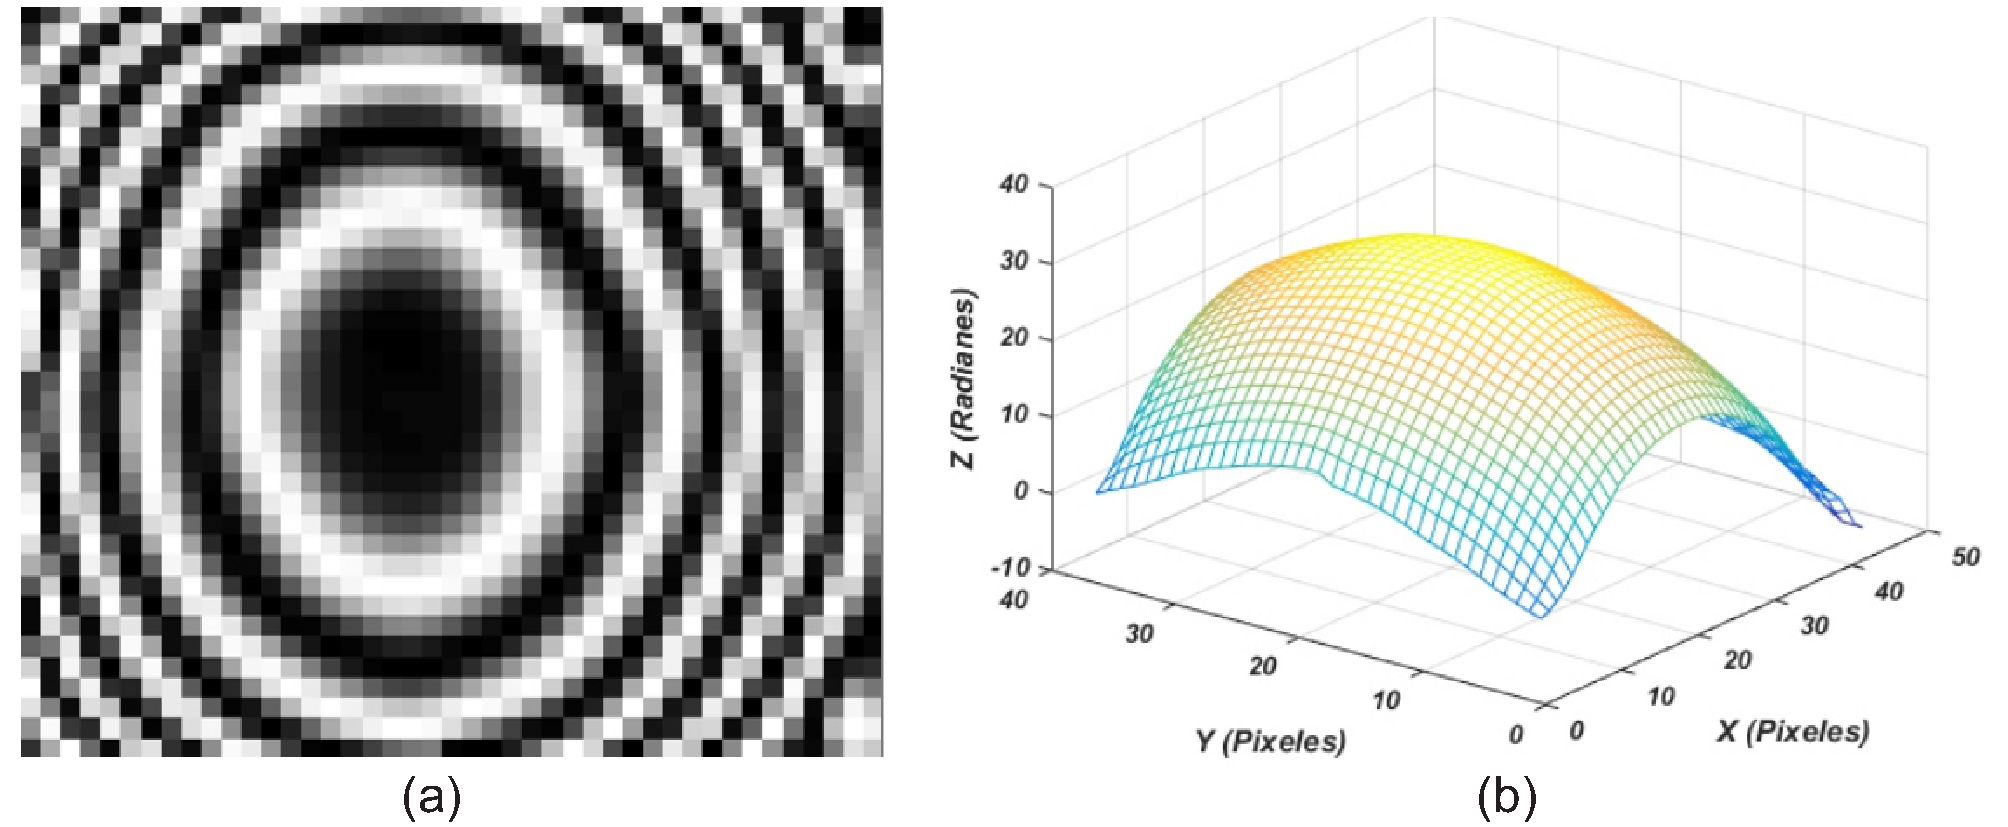
\includegraphics[width=10cm]{fig9}
\caption{(a) Fringe pattern generated from the calculated phase field by the method. (b) Phase map recovered during the demodulation process.}
\label{Fig9}
\end{figure}

The third fringe pattern used to test the model corresponds to a real shadow Moire application (Figure \ref{Fig10}a), which a low-pass filter is applied to eliminate the high frequencies produced by the grid. The original image was reduced to a resolution of 35 x 41 pixels and binarized using Otsu method to serve as an input to the algorithm (Figure \ref{Fig10}b) , which was partitioned into windows with a maximum number of fringes equal 4.
 
\begin{figure}[ht!]
\centering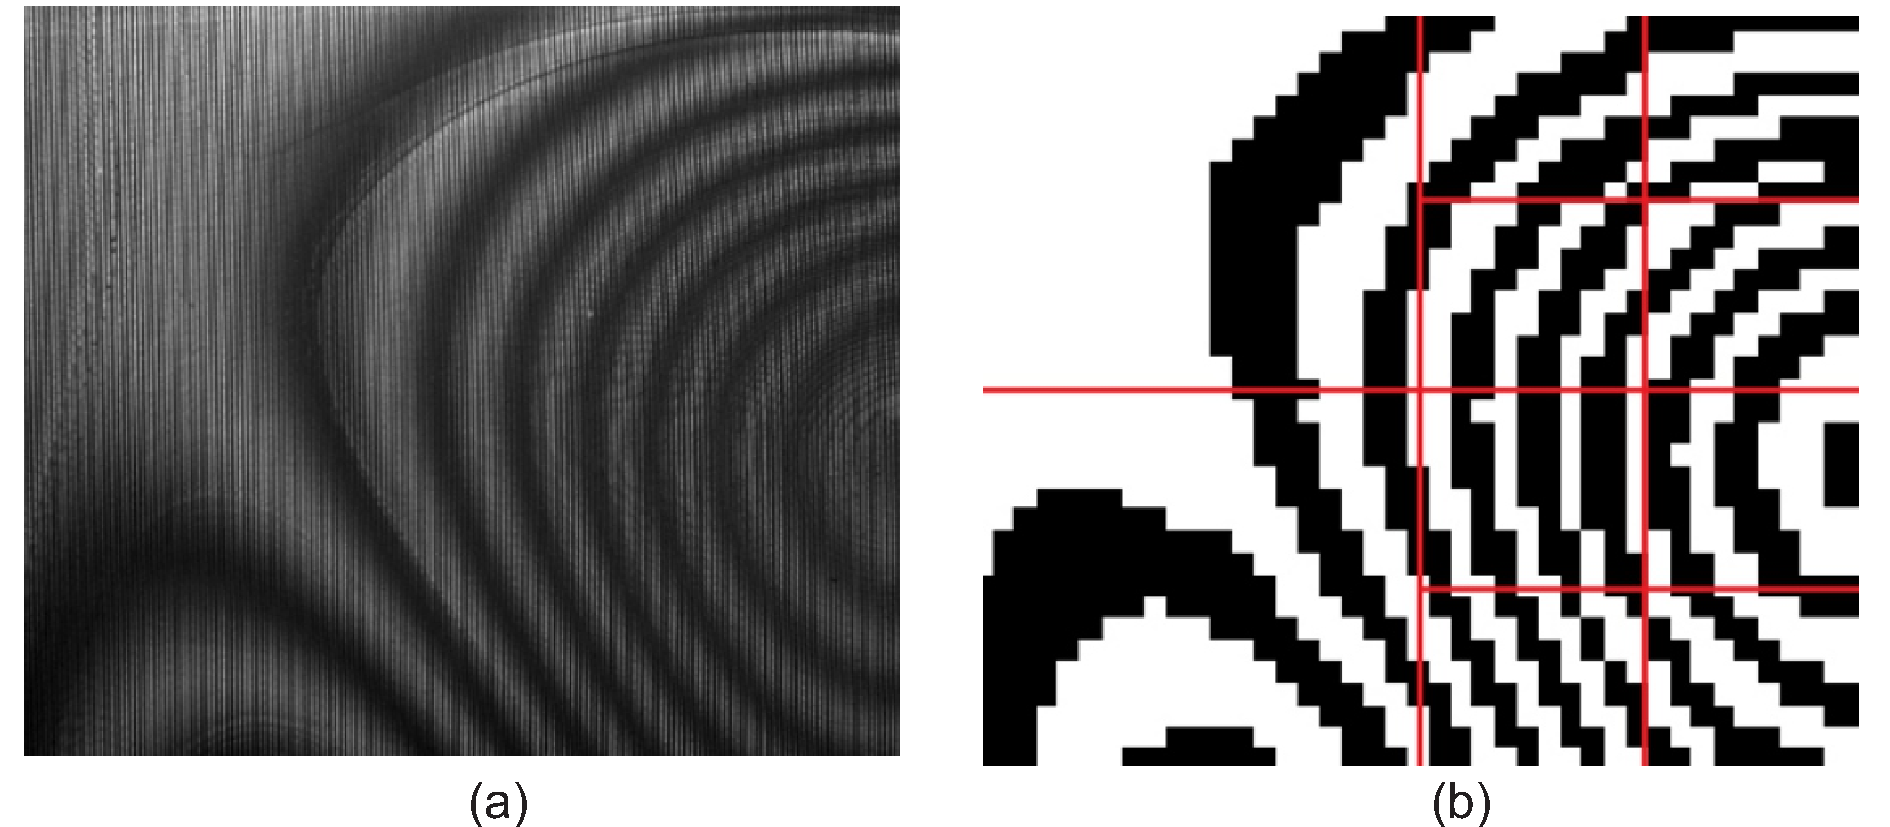
\includegraphics[width=10cm]{fig10}
\caption{(a) Original shadow moire fringe pattern with resolution of 831 $\times$ 971 pixel. (b) Independent windows partition carried out by IPA with resolution of 35 $\times$ 41 pixels.}
\label{Fig10}
\end{figure}

The SA algorithm needed 200 iterations and 50 neighbors in each loop to adjust a third-degree polynomial to each window and it took 65 seconds to get the solution. The initial temperature and the softness factor was the same configuration as the second interferogram to get the phase map. The resulting  graph obtained by this method is shown in the Figure \ref{Fig11}.

\begin{figure}[ht!]
\centering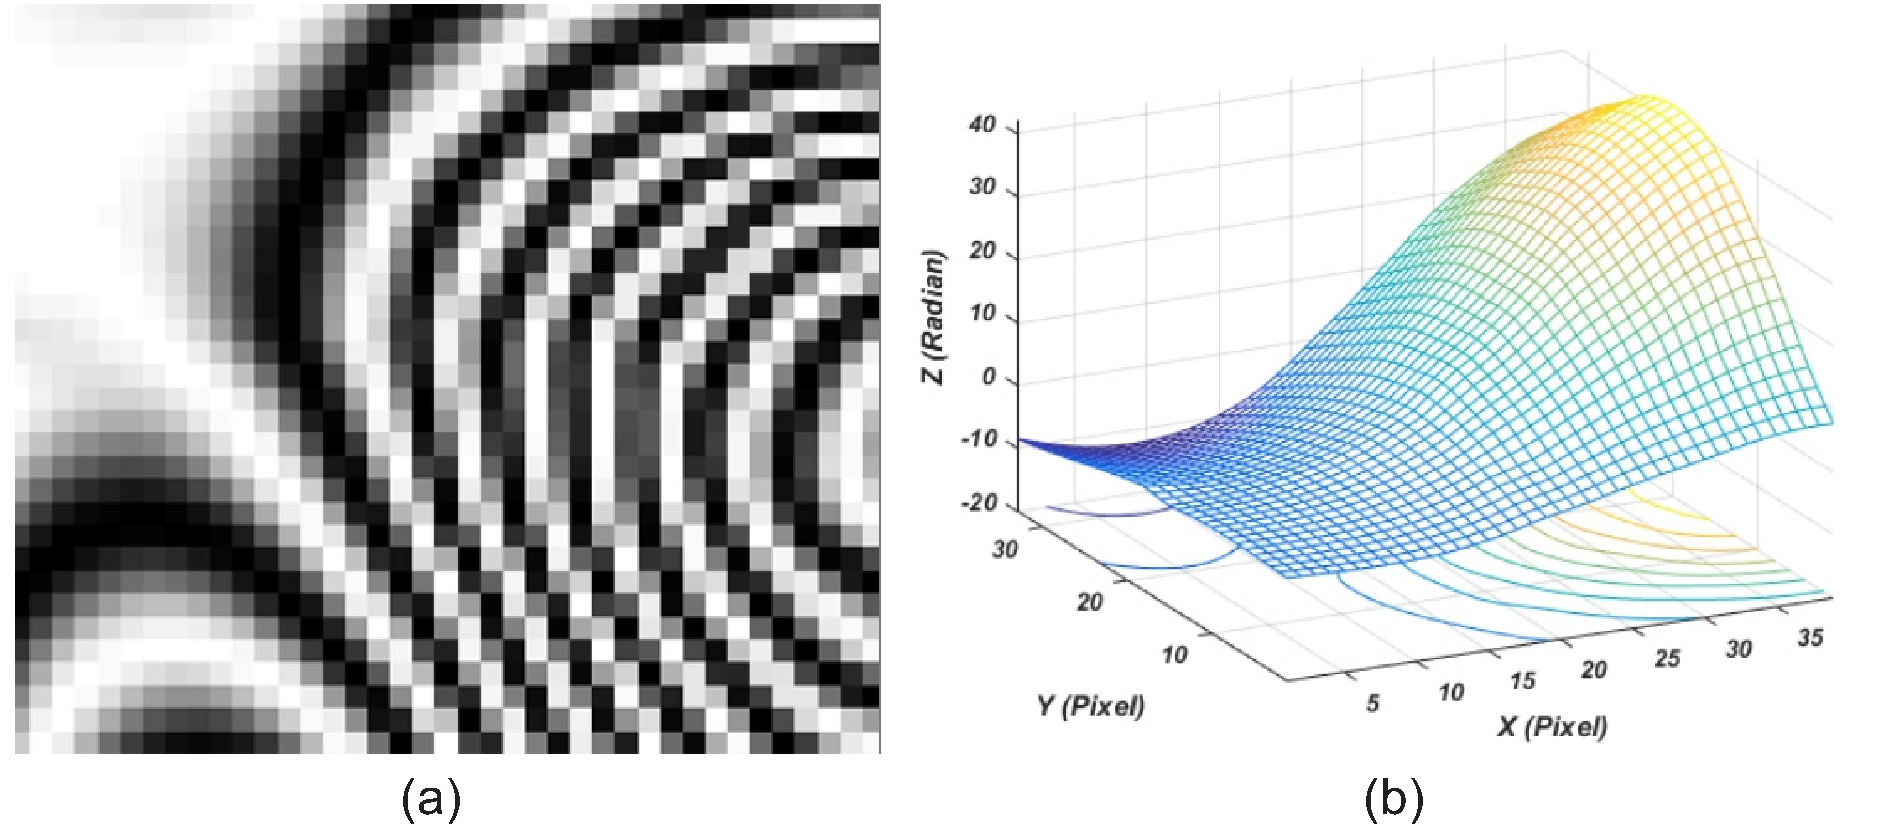
\includegraphics[width=10cm]{fig11}
\caption{(a) Fringe image obtained from the method proposed. (b) Phase map recovered from the interferogram of the Figure \ref{Fig10}b.}
\label{Fig11}
\end{figure}

The fourth test corresponds to an experiment of Digital Holography Interferometry (DHI), which can be found in the book \cite{rastogi2014phase}, by Pramod Rastogi and Erwin Hackin the chapter Local Polynomial Phase Modeling and Estimation. After the pre-processing process of the input signal to eliminate the noise produced by the experiment, the interferogram reduced to a resolution of $40\times40$ pixels to make the search process faster and more viable. Finally,the interferogram is binarized to ensure that the amplitude and the background terms remain constant. Figure \ref{Fig12} shows the pre-processing of the images, and the result after applying the partitioning algorithm with a maximum number of fringes equal to 3.

\begin{figure}[ht!]
\centering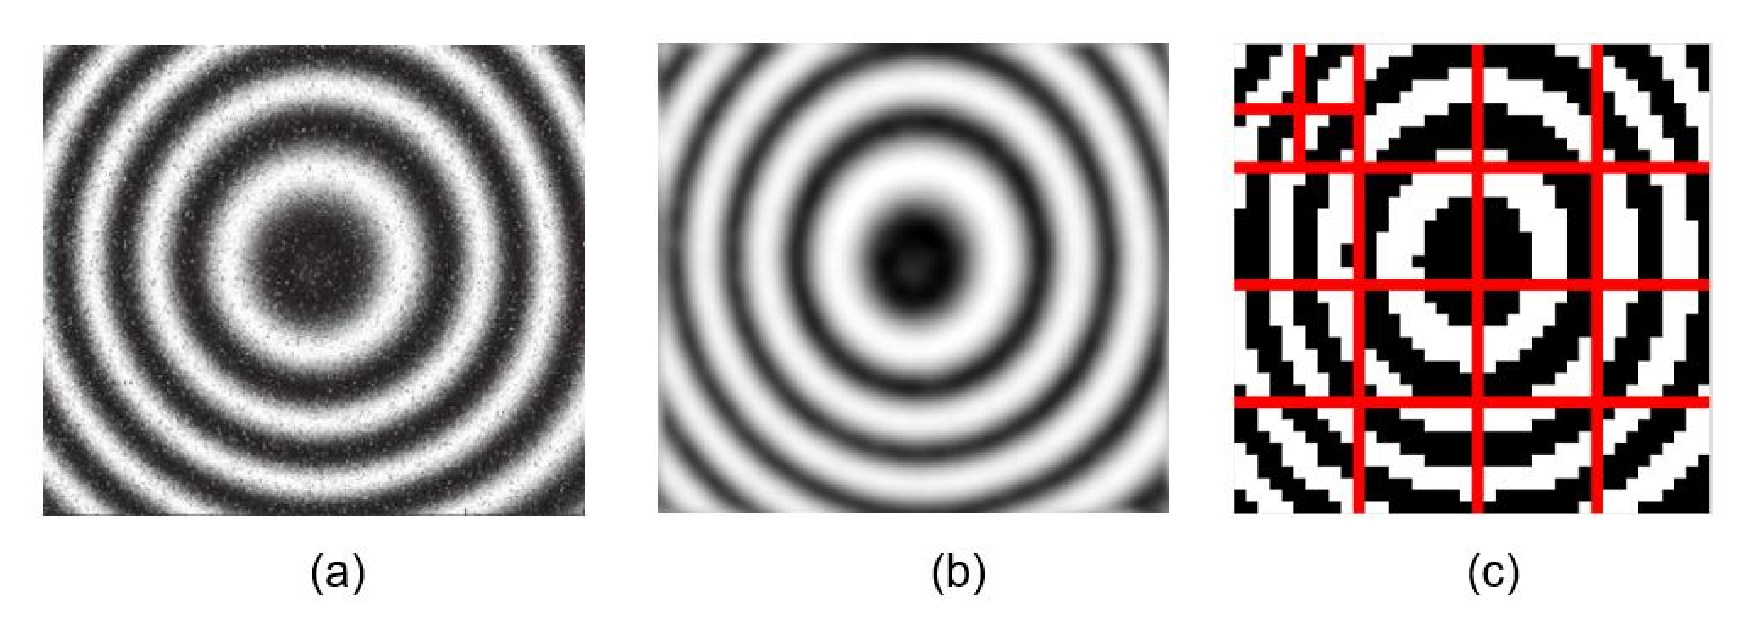
\includegraphics[width=10cm]{fig12}
\caption{(a) Experimental Fringe pattern with resolution of $500\times 500$ pixels. (b) Filtered fringe pattern. (c) c)	Binary and partitioned fringe pattern with a resolution of $40 \times 40$ pixels.}
\label{Fig12}
\end{figure}

The SA method was applied to each window with a configuration of $500$ iterations, $75$ neighboring solutions generated in each temperature interval, the smoothness factor employed was $5$  and the initial temperature was 9000 units respectively. The time consumed by the algorithm to obtain the phase map was only 67 seconds, using a second degree polynomial. Taking advantage of one of the benefits of the method with the phase in low resolution, we can make a reverse process to obtain the phase in the original resolution. The results are shown in the Figures \ref{Fig13}.

\begin{figure}[ht!]
\centering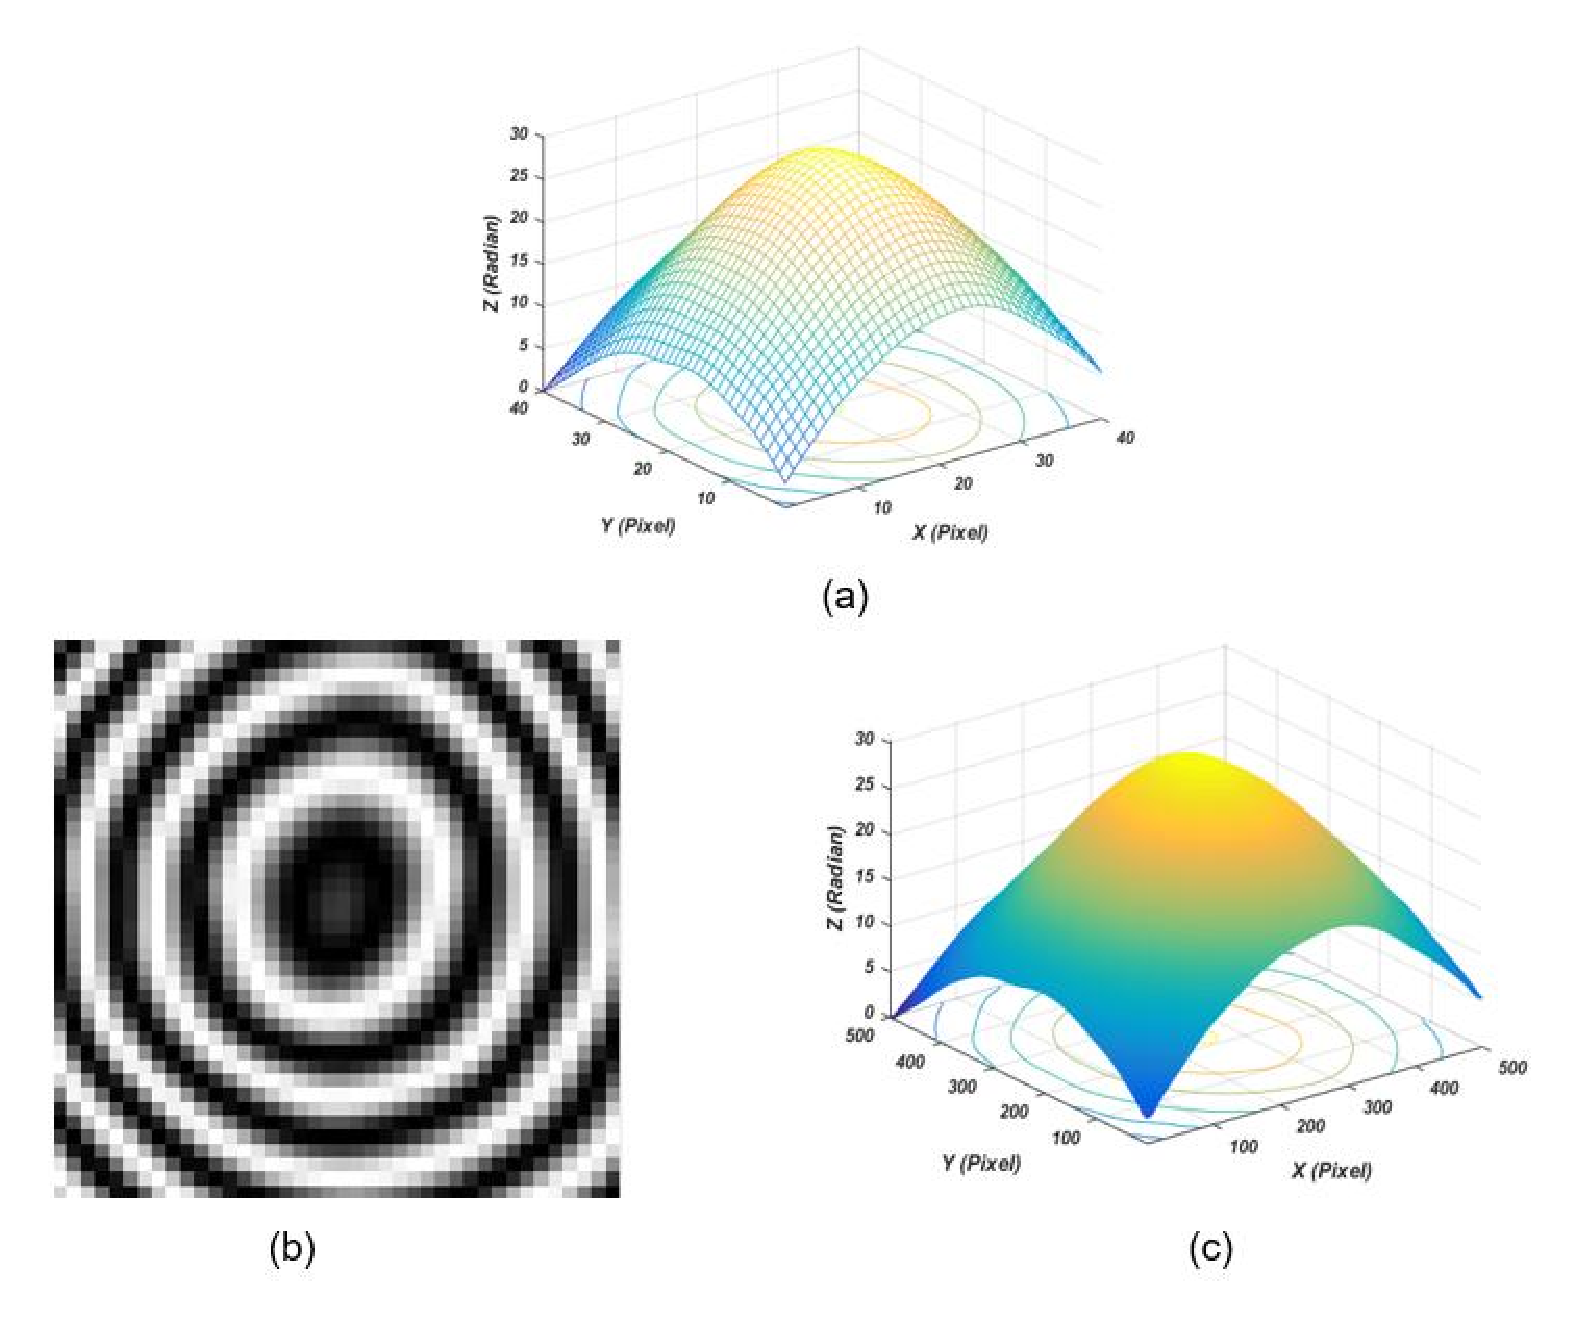
\includegraphics[width=10cm]{fig13}
\caption{(a) Recovered phase map with resolution of $40\times40$ pixels. (b) Recovered fringe pattern. (c) Recovered phase map in original resolution.}
\label{Fig13}
\end{figure}

The fifth experiment corresponds to a real interferogram, which presented a greater amount of noise, consequence that was obtained from a Spekle Interferometry experiment. The results of applying the algorithm are shown in Figure \ref{Fig14}.

\begin{figure}[ht!]
\centering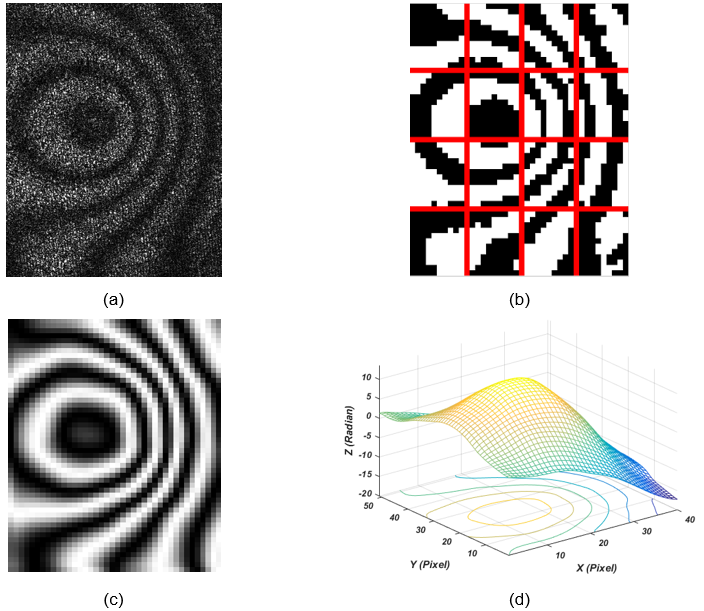
\includegraphics[width=10cm]{fig14}
\caption{Original interferogram with resolution of $390\times307$ pixels. b)Filtered and partitioned fringe pattern recovered in low resolution. c) Fringe pattern recovered. d) Phase map recovered.}
\label{Fig14}
\end{figure}

The proposed method evolved during 200 iterations to fit a second-degree polynomial to each sub-image in a period of 33 seconds. Seventy five neighbors were generated in each iteration, the initial temperature used was 9000, and the softness factor was 5. 

In light of the performed comparison, it may be suggested that the proposed method is able to find the phase map even when the Nyquist criterion is not fulfilled.

\section{Conclusions}
A proposed technique for demodulating a single interferogram using SA is presented. This model establishes a new design to partition the interferogram automatically using a recursive method that stores in a quad tree data structures the subimages with a limit of fringes in each partition. This partition allows to reduce the complexity of the windows and to make more viable the search of the algorithm of optimization. In addition, it improves the window unification method when using cubic tracing mediating approaches, consequently, this will lead to the elimination of overlapping regions and thus avoid multiple demodulation of border regions.

Six independent experiments were carried out to approximate the phase by means of polynomial functions. The first and the second images corresponded a computer simulation image with a full range of spatial frequencies and the last were experimentally obtained using a Shadow Moire technique.

Although, the main limitation of the model is with respect to the configuration of the input parameters of the algorithm, because as in any optimization model it is necessary to determine a suitable configuration, to find a feasible solution; the experimental results demonstrate the simplicity, speed and efficiency of the proposed method in comparison with other models that use optimization algorithms.

On the other hand, the great advantage of this model is that one can use the prior knowledge of the shape of the object, which opens up the possibility to use a better adapted parametric function rather than a polynomial function. Finally, we highlight the possibility of success of this technique in interferograms in which other approaches are unable to recover the phase, like the FM and PS method, where the former is unable to demodulate a closed fringes pattern and the latter needs more of an outdated image at a known angle, which brings as a disadvantage that it cannot be used in transitory events. This work demonstrates the metaheuristics recovery capacity when the resolution of the interferogram is relatively low and when Nyquist criterion is not satisfied.

\section*{Acknowledgments}
The authors thankfully acknowledge computer resources, technical advise and support provided by Laboratorio Nacional de Superc\'omputo del Sureste de M\'exico, a member of the CONACYT national laboratories, with project No. 201801048n. We also would like to thank PhD. Stephen Jones Barigye for his help during the writing process of this work.


\section*{References}

\bibliography{mybibfile}

\end{document}